
\section{Teori}

    \textbf{Motivasjon og sammenheng:} For å forstå hvorfor det er en grense på 100 meter for ethernet-kabler, og hvordan signaler dempes og forvrenges i slike kabler, må vi bruke telegraflikningen. Denne beskriver hvordan elektriske signaler forplanter seg i transmisjonslinjer, og gir oss verktøyene til å analysere tap, dispersjon.

\subsection{Fourierrekker}

Mange signaler kan brytes ned i sine frekvenskomponenter ved hjelp av Fourier-analyse. Dette er spesielt nyttig i signalbehandling og for å forstå hvordan ulike frekvenser påvirkes av transmisjonslinjen. Vi bruker Fourier-rekker for endelige intervaller (Dirichlet/Neumann). ethernet-signaler kan sees på som en sekvens av pulser (bitstrøm), som i praksis kan betraktes som et periodisk pulstog. Dette gjør at Fourierrekker er et naturlig verktøy for å analysere slike signaler i frekvensdomenet, siden pulstoget kan uttrykkes som en sum av sinus- og cosinuskomponenter.\\[1em]
en periodisk funksjon $f(t)$ med periode $T$ kan uttrykkes som en Fourier-rekke:
\begin{equation}
f(t) = a_0 + \sum_{n=1}^{\infty} \left( a_n \cos\left(\frac{2\pi n t}{T}\right) + b_n \sin\left(\frac{2\pi n t}{T}\right) \right)
\end{equation}
med koeffisienter gitt ved:
\begin{align*}
a_0 &= \frac{1}{T} \int_{0}^{T} f(t) \, dt \\
a_n &= \frac{2}{T} \int_{0}^{T} f(t) \cos\left(\frac{2\pi n t}{T}\right) dt \\
b_n &= \frac{2}{T} \int_{0}^{T} f(t) \sin\left(\frac{2\pi n t}{T}\right) dt
\end{align*}
I Komplekse form:
\begin{equation}
f(t) = \sum_{n=-\infty}^{\infty} c_n e^{i \frac{2\pi n t}{T}}, \quad \text{der} \quad c_n = \frac{1}{T} \int_{0}^{T} f(t) e^{-i \frac{2\pi n t}{T}} dt
\end{equation}
I dette prosjektet vil vi bruke Fourier-analyse for å dekomponere ethernet-signaler i sine frekvenskomponenter, slik at vi kan studere hvordan hver komponent påvirkes av transmisjonslinjens egenskaper.
Ved å gjennomføre målinger for forskjellige kabellengder, kan vi sammenligne de målte dataene med de teoretiske prediksjonene basert på Fourier-analyse og telegraflikningen.
Vi får da overføringsfunksjonen for kabelen.
\begin{equation}
    H(f) = \frac{V_{out}(f)}{V_{in}(f)}
\end{equation}
Som beskriver hvordan signalet endres i frekvensdomenet når det passerer gjennom kabelen.
Denne analysen hjelper oss å forstå hvordan ulike frekvenskomponenter dempes og forvrenges, noe som er avgjørende for å forklare begrensningen på kabelens lengde.
Setter vi inn overførsingsfunksjonen i komplekse Fourier-rekken, kan vi modellere hvordan hele signalet endres når det går gjennom kabelen.
\begin{equation}
    f_{out}(t) = \sum_{n=-\infty}^{\infty} H\left(\frac{n}{T}\right) c_n e^{i \frac{2\pi n t}{T}}
\end{equation}
\subsection{Telegraflikningen og transmisjonslinjer}
en transmisjonslinje kan beskrives ved fire per-enhet-lengde parametre:
\begin{itemize}
    \item $R$ \, [$\Omega$/m] \,-- motstand (ledertap),
    \item $L$ \, [H/m] \,-- induktans (magnetisk lagring),
    \item $C$ \, [F/m] \,-- kapasitans (elektrisk lagring),
    \item $G$ \, [S/m] \,-- ledningsevne (lekkasjetap).
\end{itemize}
Ved å kombinere Kirchhoffs lover med disse parameterne utledes telegrafligningen, som beskriver spenning og strøm som funksjon av både posisjon og tid langs kabelen. For spenningen $u(x,t)$ kan den skrives på formen:
\begin{equation}
    u_{tt} + (RG + LC)u_t + RG\,u = c^2 u_{xx}, \qquad c = \frac{1}{\sqrt{LC}} ,
\end{equation}
der $u(x,t)$ er spenningen langs kabelen og $c$ er utbredelseshastigheten i kabelen.  
Denne ligningen viser at et signal ikke bare forplanter seg med en hastighet bestemt av $L$ og $C$, men også blir dempet og forvrengt på grunn av $R$ og $G$. Resultatet er at høyfrekvente komponenter i signalet svekkes og spres mer enn lave frekvenser, noe som over tid fører til \emph{demping og dispersjon}.  
ethernet-signaler består ikke av rene sinusbølger, men av pulser med et bredt spekter av frekvenser. Mens fourier-analyse kan hjelpe oss  å utrykke signalet som en sum av ulike frekvenskomponenter, gir telegrafligningen oss verktøy til å studere hvordan hver enkelt komponent påvirkes. Dermed kan vi forklare hvorfor en grense på omtrent 100 meter er praktisk: etter denne lengden er tapet og forvrengningen så store at signalet ikke lenger kan tolkes pålitelig av mottakeren.


\subsubsection{R - Resistans}
Resistans per lengde $[\Omega/\mathrm{m}]$ er den ohmske motstanden i lederen. Den skyldes av materialets resistivitet og ledertverrsnitt, og øker med temperatur. Motstanden øker dempingen og rekkevidden til signalet. I telegrafligningen bidrar R direkte til tidsdemping av både strøm og spenning.

\subsubsection{L - Induktans}
Induktansen per lengde $[\mathrm{H}/\mathrm{m}]$ er magnetisk lagring av energi rundt lederen når strømmen endres, per meter kabel. Sammen med kapasitans vil denne bestemme farten på signalet i kabelen. I linjemodellen er induktans i seriekobling.

\subsubsection{C - Kapasitans}
Kapasitans per lengde $[\mathrm{F}/\mathrm{m}]$ er elektrisk lagring av energi i feltet mellom leder og referanse, per meter. Sammen med induktans har kapasitans påvirkning på fart. I linjemodellen er dette en gren til jord, den trekker ladning når spenningen endres.

\subsubsection{G - Ledningsevne}
Ledningsevnen per meter $[\mathrm{S}/\mathrm{m}]$ beskriver det dielektriske taper gjennom isolasjonen til jord, per meter. Det påvirker signalet i form av å øke dempingen fordi energi vil lekke i dielektrikumet. Høy fuktighet eller dårlig isolasjon vil svekke ledningsevnen. Ledningsevnen opererer i parallelt med kapasitansen i linjemodellen.









\subsubsection{Utledning av telegraflikningen}
Telegraflikningen kan utledes ved å analysere en liten del av transmisjonslinjen, som vist i figuren nedenfor. Vi betrakter et segment av linjen med lengde $\Delta x$, og bruker Kirchhoffs spennings- og strømlov for å sette opp differensialligninger for spenning og strøm.
\begin{figure}[h]
    \centering
    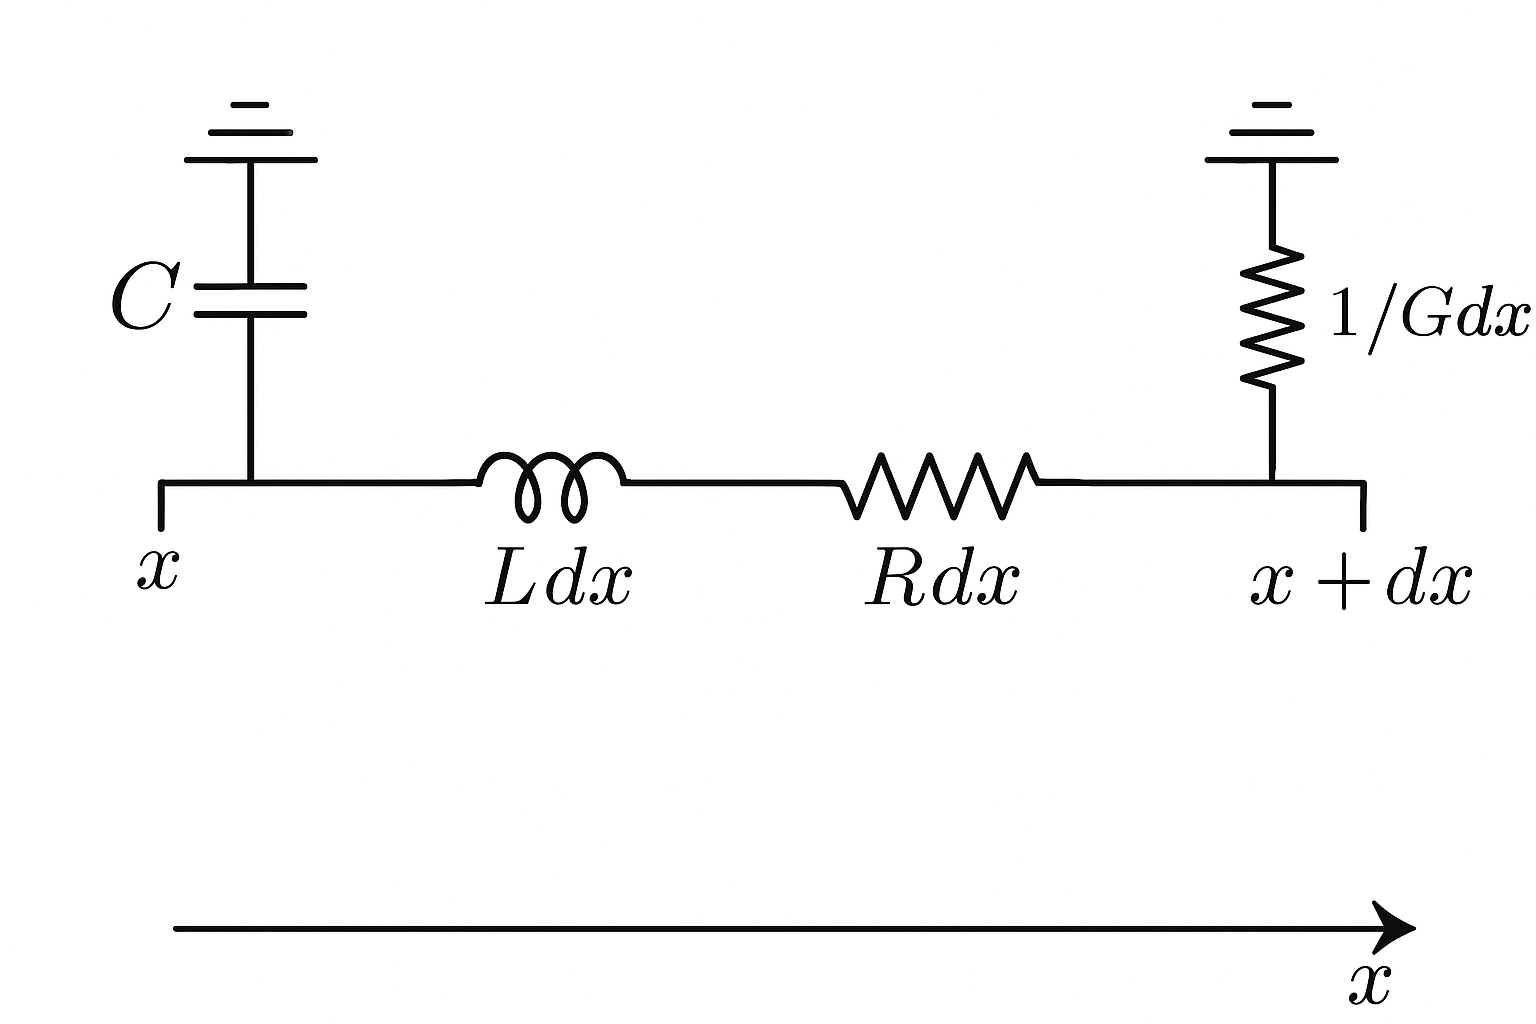
\includegraphics[width=0.6\textwidth]{Media/telegraflinje.png}
    \caption{elementær segment av en transmisjonslinje med per-enhet-lengde parametere.}
    \label{fig:transmission_line_segment}   
\end{figure}
Ved å anvende Kirchhoffs spenningslov på segmentet får vi:
\[
    u(x,t) - u(x+\Delta x,t) = R \Delta x \cdot i(x,t) + L \Delta x \cdot \frac{\partial i(x,t)}{\partial t} .
\]
Ved å la $\Delta x \to 0$ får vi den første differensialligningen:
\begin{equation}
    \frac{\partial u(x,t)}{\partial x} = -R i(x,t) - L \frac{\partial i(x,t)}{\partial t} . 
\end{equation}
Tilsvarende, ved å bruke Kirchhoffs strømlov, får vi:
\[
    i(x,t) - i(x+\Delta x,t) = -G \Delta x \cdot u(x,t) - C \Delta x \cdot \frac{\partial u(x,t)}{\partial t} .
\]
Igjen, ved å la $\Delta x \to 0$ får vi den andre differensialligningen:
\[
    \frac{\partial i(x,t)}{\partial x} = -G u(x,t) - C \frac{\partial u(x,t)}{\partial t} .
\]
Ved å derivere den første ligningen med hensyn på $x$ og den andre med hensyn på $t$, og deretter eliminere $i(x,t)$, får vi telegraflikningen for spenningen:
\[
    u_{tt} + (RG + LC)u_t + RG\,u = c^2 u_{xx}, \qquad c = \frac{1}{\sqrt{LC}} .
\]
Dette kan vi skrive som:
\begin{equation}
    u_{tt} + (\alpha + \beta)u_t + \alpha \beta u = c^2 u_{xx}, \qquad c = \frac{1}{\sqrt{LC}} ,
    \label{eq:telegraflikningen}
\end{equation}
der vi har definert:
\[
    \alpha = \frac{R}{L}, \qquad \beta = \frac{G}{C} .
\]
Dette er en dampet bølgeligning som beskriver hvordan spenningen forplanter seg langs transmisjonslinjen, med demping og forvrengning bestemt av parametrene $R$, $L$, $C$, og $G$.



\subsubsection{Propagerende løsning og overføringsfunksjon}

I forrige del utledet vi telegraflikningen for spenning langs en kabel uttrykt ved de per-lengde-parametrene $R, L, G, C$ som beskriver hvordan spenningen varierer både i tid og rom \eqref{eq:telegraflikningen}. Denne likningen er en såkalt bølgelikning med demping. Vi forventer derfor at løsningene skal ha bølgekarakter som oscillerer i tid og samtidig forplanter seg langs kabelen. For å fange dette opp antar vi en løsning på formen
\begin{equation}
V(x,t) = \Re\!\left\{ U e^{j\omega t - \gamma(\omega)x} \right\}.
\label{eq:harm-ansatz}
\end{equation}
Her har vi valgt tre elementer:
\begin{itemize}
    \item \textbf{Tidsdelen $e^{j\omega t}$:} beskriver en harmonisk oscillasjon i tid. At vi bruker den 
    komplekse eksponentialen i stedet for $\cos(\omega t)$ eller $\sin(\omega t)$ skyldes at dette 
    gjør beregningene enklere. Til slutt tar vi realdelen for å hente ut det fysiske signalet.
    \item \textbf{Romdelen $e^{-\gamma x}$:} beskriver hvordan signalet utvikler seg langs kabelens lengde. 
    Hvis $\gamma$ er reell, betyr dette ren demping. Hvis $\gamma$ er imaginær, betyr det ren faseforskyvning. 
    I praksis er $\gamma$ kompleks, slik at vi får begge deler.
    \item \textbf{Kompleks amplitude $U$:} setter størrelsen og fasen på bølgen.\\
\end{itemize}
Dette kalles en \emph{harmonisk ansats}. Den er valgt fordi vi vet fra Fourier-teori at alle signaler 
kan bygges opp som en sum av slike harmoniske komponenter. Når vi kjenner kabelens respons på en frekvens, 
kan vi utvide til vilkårlige signaler. Setter vi \eqref{eq:harm-ansatz} inn i telegraflikningen \eqref{eq:telegraflikningen}:
\[    
    V_{tt} + (\alpha + \beta)V_{t} + \alpha \beta V = c^2 V_{xx}.
\]
Ser vi at den tidslige avledningen bare gir faktorer av $j\omega$:
\[
    V_{t} = j\omega V, \quad V_{tt} = -\omega^2 V,
\]
og den romlige avledningen gir faktorer av $\gamma$:
\[
    V_{x} = -\gamma V, \quad V_{xx} = \gamma^2 V.
\]
Som gir oss:
\[    
-\omega^2 V + j\omega(\alpha+\beta)V + \alpha \beta V = c^2 \gamma^2 V.
\]
Etter innsetting og forenkling står vi igjen med sammenhengen
\[
c^2 \gamma^2(\omega) = \alpha \beta - \omega^2 + j\omega(\alpha+\beta).
\]
Dette er en såkalt \emph{dispersjonsrelasjon}, som forteller hvilke kombinasjoner av 
frekvens $\omega$ og bølgetall $\gamma$ som er mulige. Vi kan løse for $\gamma$ og får
\[
\gamma(\omega) = \frac{1}{c}\sqrt{\alpha\beta - \omega^2 + j\omega(\alpha+\beta)}.
\]
Setter vi inn definisjonene på $\alpha,\beta$ og $c$, kan dette skrives på den standardformen
som brukes i transmisjonslinjeteori:
\begin{equation}
\;\gamma(\omega) = \sqrt{(R+j\omega L)(G+j\omega C)}\;
\end{equation}
Dette uttrykket viser tydelig hvordan både ledertap ($R$) og dielektriske tap ($G$) bidrar 
til at signalet dempes, mens $L$ og $C$ bestemmer hastigheten til bølgen. Vi kan også uttrykke $\gamma$
i form av sin reelle og imaginære del:
\[
\gamma(\omega) = \alpha_p(\omega) + j\beta_p(\omega).
\]
Her har $\alpha_p(\omega)$ enheten Np/m (neper per meter) og forteller hvor raskt amplituden 
avtar med lengden, mens $\beta_p(\omega)$ har enheten rad/m og forteller hvor raskt fasen 
øker langs kabelen. Fra $\beta_p$ kan vi utlede bølgens fasehastighet:
\[v_p = \frac{\omega}{\beta_p}\]
og dermed hvor stor tidsforsinkelse signalet får etter en viss lengde.\\[1em]
Hvis vi nå ser på en kabel av lengde $l$, vil en harmonisk komponent ved frekvens $\omega$ 
endres med faktoren
\begin{equation}
H(\omega,l) = e^{-\gamma(\omega)l} = e^{-\alpha(\omega)l}\,e^{-j\beta(\omega)l}
\end{equation}
Dette er kabelens \emph{overføringsfunksjon}. 
Den kan forstås slik:
\begin{itemize}
    \item $e^{-\alpha l}$: amplituden reduseres eksponentielt med lengden, 
    \item $e^{-j\beta l}$: signalet forskyves i fase, tilsvarende en tidsforsinkelse.\\[1em]
\end{itemize}
Så langt har vi bare sett på en harmonisk bølge. Men i praksis er alle signaler satt sammen av mange slike. 
et vilkårlig innsignal kan skrives som en Fourier-rekke:
\[
f_{\text{in}}(t) = \sum_n c_n e^{j\omega_n t}.
\]
etter kabelen vil hver komponent være påvirket av $H(\omega_n,l)$, og vi får
\[
f_{\text{out}}(t) = \sum_n H(\omega_n,l)\,c_n e^{j\omega_n t}.
\]
Dermed virker kabelen som et frekvensavhengig filter: lave frekvenser slipper nesten uendret gjennom, 
mens høye frekvenser dempes kraftig. For firkantsignaler betyr dette at de skarpe kantene, 
som består av mange høye frekvenser, gradvis blir avrundet etter hvert som lengden øker. 
Det er nettopp dette vi kan observere i laboratoriet når vi sender firkantpulser gjennom en ethernet-kabel.


\subsection{Metoder og praktisk relevans}

(a) \textit{Fourierrekker:} Analytisk på $[0,L]$ (m/Dirichlet) for å vise $\alpha=\beta$-tilfellet.\\
\dots
\clearpage
\subsection{Dispersjon}

Dispersjon betyr at ulike frekvenskomponenter i en bølge forplanter seg med forskjellig hastighet. 
I telegrafligningen oppstår dette fordi bølgefarten $v_n$ avhenger av frekvensen og parameterne 
$R$, $L$, $C$ og $G$. 

Konsekvensen er at et signal som består av mange frekvenser (for eksempel en skarp puls) gradvis 
forvrenges når det forplanter seg. Dette er en sentral utfordring i signaloverføring: skarpe signaler 
blir bredere og mister form over tid. 
\dots

\subsection{Oppsummering og kobling til prosjektet}

Teorien over forklarer hvorfor signaler i lange kabler dempes og forvrenges, og gir oss verktøyene til å analysere dette både analytisk og numerisk. Dette er avgjørende for å forstå hvorfor det er en 100 m-grense for ethernet-kabler. I det videre arbeidet skal vi først gjennomføre praktiske målinger, og deretter \textcolor{red}{numeriske simuleringer} (kanskje), slik at begge kan sammenlignes med de teoretiske resultatene for å se hvordan modellen stemmer med virkeligheten.
